\documentclass[14pt,aspectratio=169,xcolor=dvipsnames,table,onlytextwidth]{beamer}
\input{macros_en}
\csname endofdump\endcsname
\title{Polyhedral Combinatorics}
\subtitle{Introduction to Computational Mathematics}
\author{Instructor: \textbf{Tasuku Soma}}

\begin{document}
\maketitle

\begin{frame}<1>[label=outline]{Outline}
\begin{tikzpicture}
    \tikzstyle{block} = [rectangle, text width=\textwidth, rounded corners, minimum height=4em]
    \tikzstyle{line} = [draw, -latex]

    \node[block,alt={<1,3->{fill=cyan!10}{fill=red!10}}] (combopt) {
        \begin{columns}
            \begin{column}{0.40\linewidth}
        \textbf{1. What is combinatorial optimization?}
            \end{column}
            \begin{column}{0.5\linewidth}
                \small
                \structure{\textbullet} What is combinatorial optimization?\\
                \structure{\textbullet} What does it mean to ``solve'' a problem?\\
                \structure{\textbullet} What is polynomial time?
            \end{column}
        \end{columns}
    };
    \node[block,alt={<1-2,4->{fill=cyan!10}{fill=red!10}}, below=.5em of combopt] (LP) {
        \begin{columns}
            \begin{column}{0.4\linewidth}
        \textbf{2. Review of linear programming}
            \end{column}
            \begin{column}{0.5\linewidth}
                \small
                \structure{\textbullet} Primal and dual problems \\
                \structure{\textbullet} Complementary slackness \\
                \structure{\textbullet} Polyhedra
            \end{column}
        \end{columns}
    };
    \node[block,alt={<1-3,5->{fill=cyan!10}{fill=red!10}}, below=.5em of LP] (TU) {
        \begin{columns}
            \begin{column}{0.5\linewidth}
        \textbf{3. Integral polyhedra and totally unimodular matrices}
            \end{column}
            \begin{column}{0.5\linewidth}
                \small
                \structure{\textbullet} Totally unimodular matrices \\
                \structure{\textbullet} Integral polyhedra \\
                \structure{\textbullet} Integral polyhedra and integrality of LP\\
            \end{column}
        \end{columns}
    };
\end{tikzpicture}%
\end{frame}

%%%%%%%%%%%%%%%%%%%%%%%%%%%%%%%%%%%%%%%%%%%%%
\section{What is combinatorial optimization?}
\againframe<2|handout:0>{outline}
%%%%%%%%%%%%%%%%%%%%%%%%%%%%%%%%%%%%%%%%%%%%%
\begin{frame}
    \frametitle{What is combinatorial optimization?}
    A methodology for finding the best solution among \alert{discrete} objects \alert{efficiently}.

    \vfill
    \begin{columns}[]
        \begin{column}{.3\textwidth}
            \centering
            
\includegraphics[width=\textwidth]{figs/network.jpg}
            Networks
        \end{column}
        \begin{column}{.3\textwidth}
            \centering
        \begin{tikzpicture}[>=latex,scale=.8]
        \foreach \i in {1,2,3} {
            \node[inner sep=0pt](v\i) at ($(0, -\i*2)$) {\coloremojiucs[scale=2]{:factory:}};
            \node[inner sep=0pt](w\i) at ($(4, -\i*2)$) {\coloremojiucs[scale=2]{:convenience_store:}};
        }
        \graph{
            {(v1), (v2), (v3)} --[complete bipartite] {(w1), (w2), (w3)}
        };
        \end{tikzpicture}
            Matchings
        \end{column}
        \begin{column}{.3\textwidth}
            \centering
            % \includegraphics[width=\textwidth]{active.pdf}
            \tikzset{block/.style={draw, thick, rectangle}}
            \begin{tikzpicture}[>=latex]
                \node[block](x1) at (0,2)  {$X_1$};
                \node[block](x2) at (0,1)  {$X_2$};
                \node[]          at (0,0)  {$\vdots$};
                \node[block](xn) at (0,-1) {$X_n$};
                \node[block](y)  at (3,0)  {$Y$};
                \begin{scope}[every path/.style={->,very thick,gray}]
                \draw (x1.east) to [bend left ] (y.west);
                \draw (x2.east) -- (y.west);
                \draw (xn.east) to [bend right] (y.west);
                \end{scope}
            \end{tikzpicture}
            Machine learning and statistics
        \end{column}
    \end{columns}
\end{frame}

\begin{frame}[t]
    \frametitle{Example: Assignment problem}
    \begin{columns}[T]
    \begin{column}{.5\textwidth}
        \begin{block}{Assignment problem}
            \structure{Input} Costs $c_{ij} \in \R$ ($1 \leq i, j \leq n$) \\
            \structure{Output} A matching with minimum total cost
        \end{block}

        \vspace{3em}
        \small
        \alert{matching}: a set of edges s.t. every vertex is incident to exactly one edge.
    \end{column}
    \begin{column}{.5\textwidth}
        \centering
        \begin{tikzpicture}[>=latex]
        \foreach \i in {1,2,3} {
            \node[inner sep=0pt](v\i) at ($(0, -\i*2)$) {\coloremojiucs[scale=2]{:factory:}};
            \node[inner sep=0pt](w\i) at ($(4, -\i*2)$) {\coloremojiucs[scale=2]{:convenience_store:}};
        }
        \graph{
            {(v1), (v2), (v3)} --[complete bipartite] {(w1), (w2), (w3)}
        };
        \path (v1)--(w1) node[midway,above,align=center]{\small Shipping cost $c_{ij}$ \\ \reflectbox{\coloremoji{🚛}}};
        \node[above=1pt of v1] {$i$};
        \node[above=1pt of w1] {$j$};

        \onslide<2->{
            \graph[edges={UniBlue,very thick}]{
                (v1) -- (w1);
                (v2) -- (w3);
                (v3) -- (w2);
            };
        }
    \end{tikzpicture}\\
    \onslide<2->{Total cost $= c_{11} + c_{23} + c_{32}$.}
    \end{column}
    \end{columns}
\end{frame}

\begin{frame}[t]
    \frametitle{Example: Traveling salesperson problem (TSP)}
    \begin{columns}[T]
    \begin{column}{.55\textwidth}
        \begin{block}{Traveling salesperson problem}
            \structure{Input} Edge costs $c_{ij} \in \R$ ($1 \leq i, j \leq n$) \\
            \structure{Output} A minimum-cost cycle visiting each vertex exactly once
        \end{block}
    \end{column}
    \begin{column}{.40\textwidth}
    \centering
    \begin{tikzpicture}[xscale=1.2,>=latex]
        \begin{scope}[every node/.style={inner sep=0pt}]
            \node(v1) at (18 :2) {\coloremoji[scale=2]{🗼}};
            \node(v2) at (90 :2) {\coloremoji[scale=2]{🏠}};
            \node(v3) at (162:2) {\coloremoji[scale=2]{🏫}};
            \node(v4) at (234:2) {\coloremoji[scale=2]{🏬}};
            \node(v5) at (306:2) {\coloremoji[scale=2]{🏝}};
        \end{scope}
        \node[above=1pt of v2] {$i$};
        \node[right=1pt of v1] {$j$};
        \graph{
            subgraph K_n[V={(v1), (v2), (v3), (v4), (v5)}];
        };
        \path (v1) -- node[midway,sloped,above,align=center]{\small Edge cost $c_{ij}$ \\ \reflectbox{\coloremoji{🚶‍♀️}}} (v2);
        \onslide<2->{
        \graph[edges={UniBlue,very thick}]{
            (v2) -> (v1);
            (v1) -> (v3);
            (v3) -> (v5);
            (v5) -> (v4);
            (v4) -> (v2);
        };
        }
    \end{tikzpicture}
    \end{column}
    \end{columns}
\end{frame}

\begin{frame}[t,label=maxcoverage]
    \frametitle{Example: Maximum coverage problem}

    \begin{columns}[T]
    \begin{column}{.55\textwidth}
        \begin{block}{Maximum coverage problem}
            \structure{Input} $V$: candidate base-station locations, $k \in \Z_+$ \\
            \structure{Output} $S \subseteq V$ with $|S| \leq k$ that maximizes the covered area
        \end{block}
    \end{column}
    \begin{column}{.40\textwidth}
    \centering
    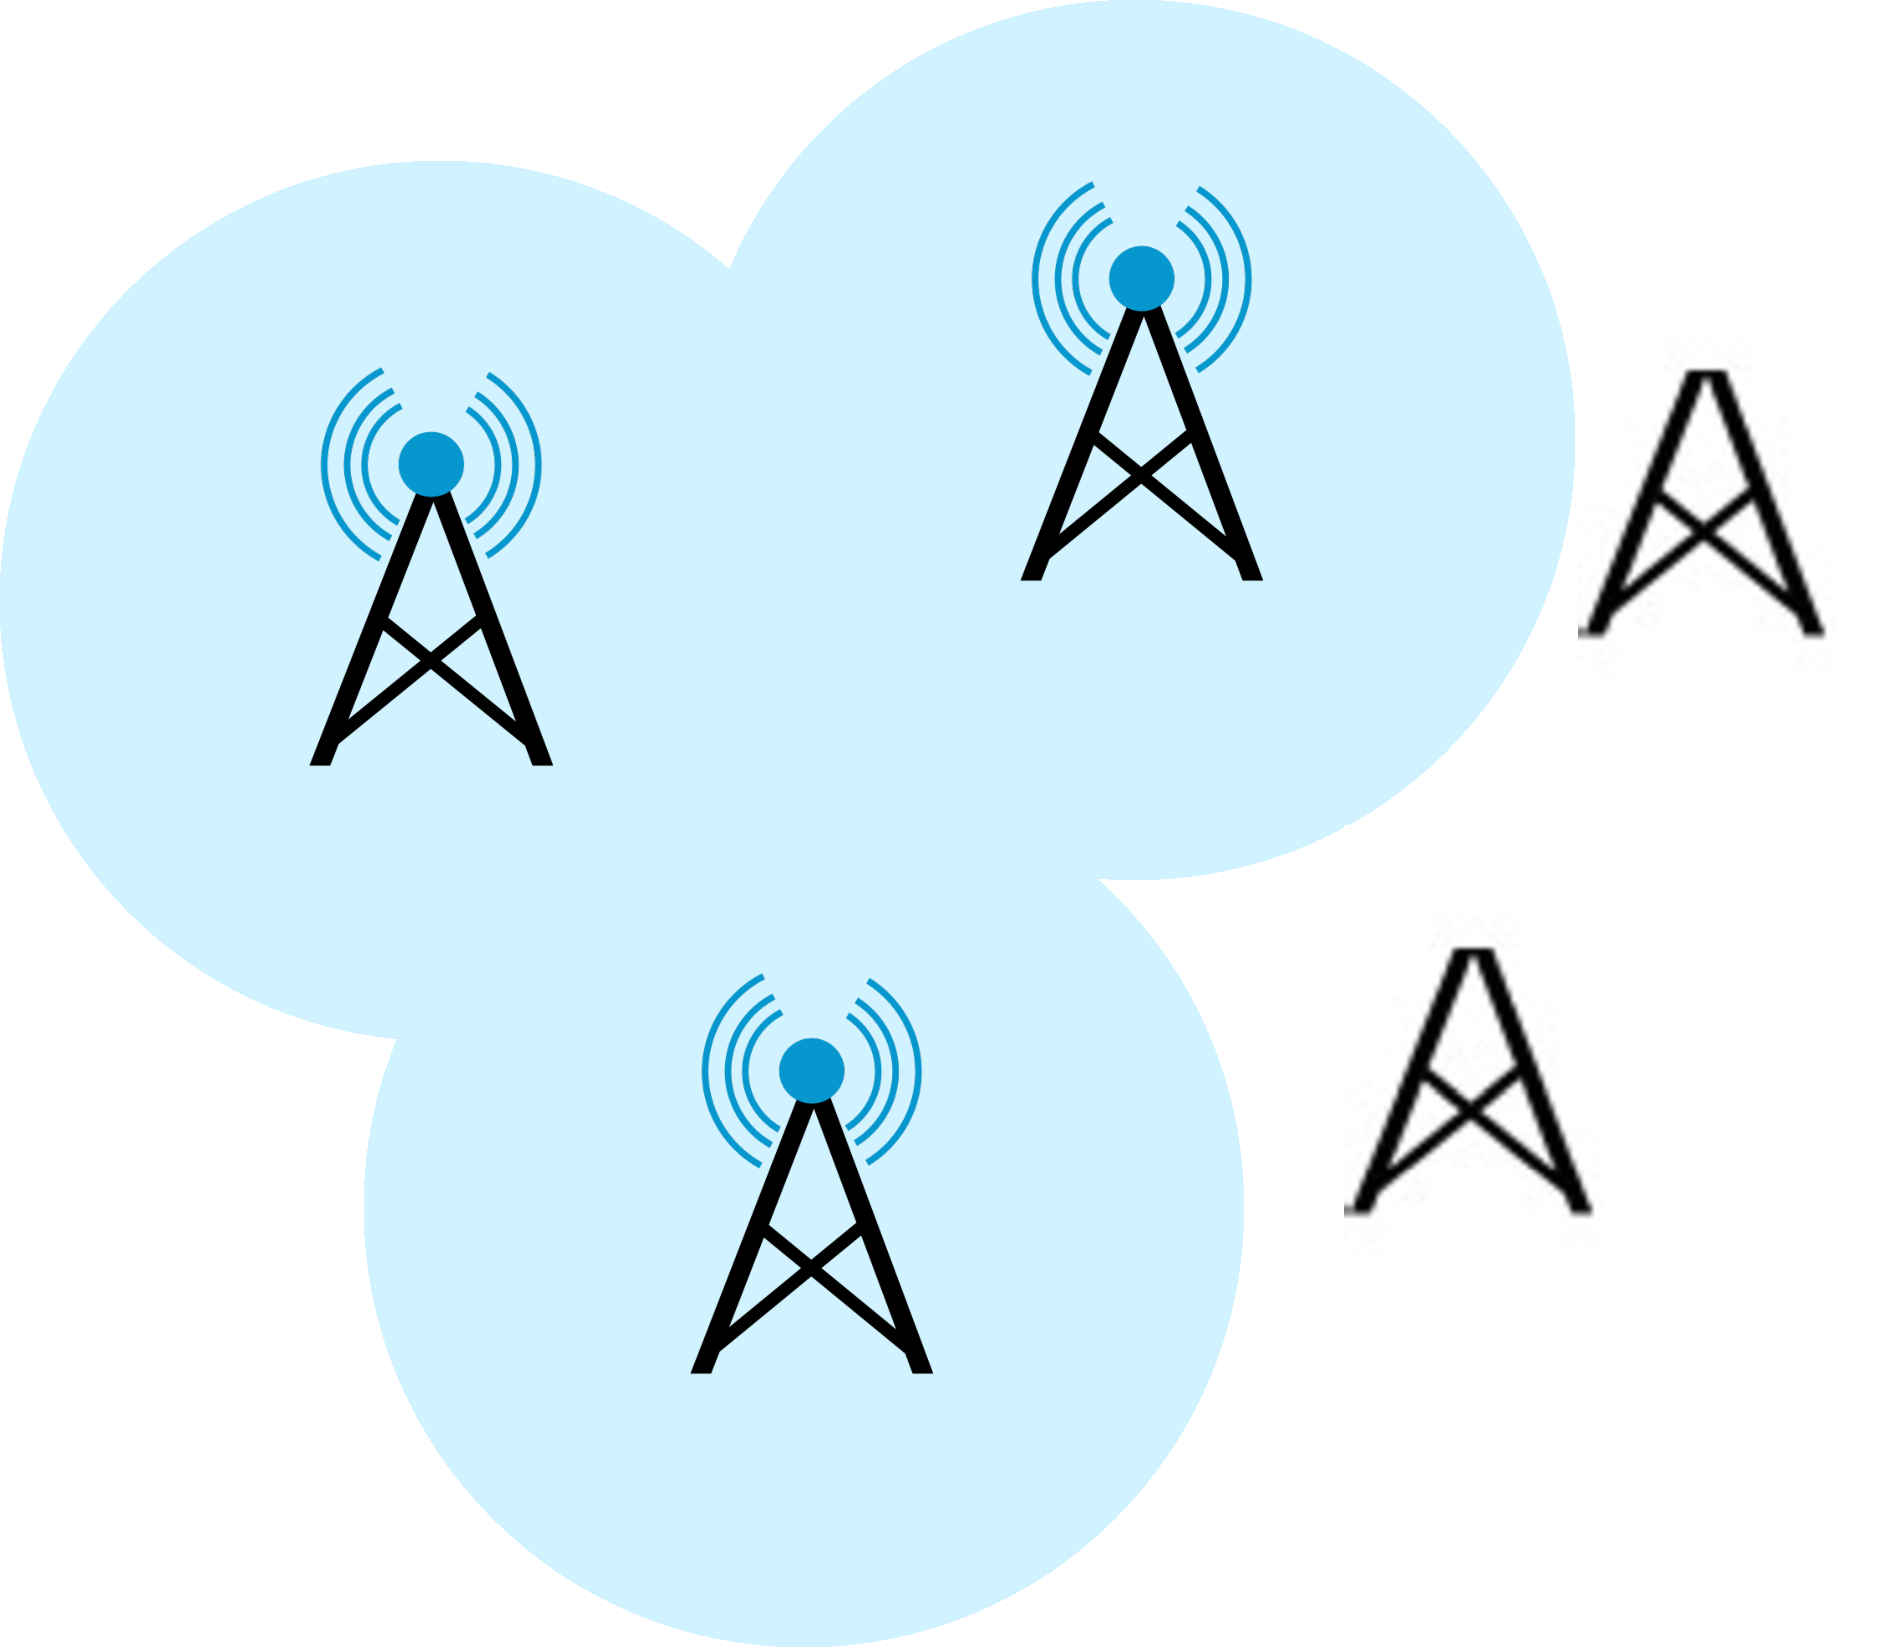
\includegraphics[width=\linewidth]{figs/coverage.pdf}
    \end{column}
    \end{columns}

\end{frame}

\begin{frame}
    \frametitle{A naive approach: Brute force search}
    Examine all solutions and choose the best one!
    \pause
    \begin{center}
        \begin{columns}[T]
        \begin{column}{.5\textwidth}
        \centering
        For TSP \\
        {\scriptsize Suppose we can examine $10^{17}$ solutions per second.}
        \rowcolors{1}{UniBlue!20}{white}

        \bigskip
        \begin{tabular}{cc}
            $\#$ of vertices $n$ & Computation time $\approx n!$ \\ \hline
            10 & $3.6 \times 10^{-11}$ sec \\
            20 & 24 sec \\
            30 & 31.68 million years
        \end{tabular}
        \end{column}
        \pause
        \begin{column}{.5\textwidth}
            \centering
            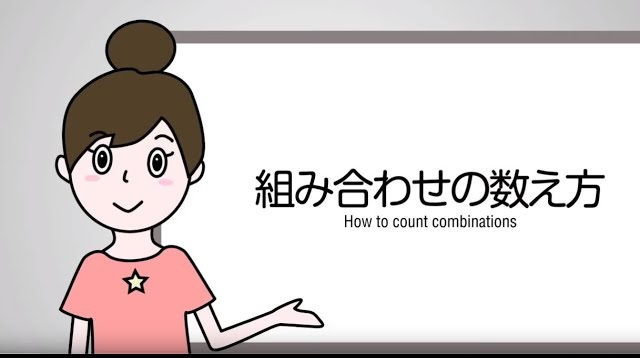
\includegraphics[width=.8\linewidth]{figs/onesan.jpg} \\
            \tiny Source: 
            \url{https://www.youtube.com/watch?v=Q4gTV4r0zRs}
        \end{column}
        \end{columns}
    \end{center}
    \pause
    This is impractical, so we need to develop more \alert{efficient algorithms}.
    \begin{center}
    \textbf{What does ``efficient'' mean?}\coloremoji[scale=1.5]{🤔}
    \end{center}
\end{frame}

\begin{frame}
    \frametitle{Time complexity of algorithms}

    \begin{block}{Time complexity of algorithms}
    The time complexity of an algorithm is the \alert{maximum} number of \alert{elementary operations} (arithmetic operations, comparisons, bit operations, \ldots) performed by it.
    \end{block}
    \pause
    \vfill
    $n$: size of input
    \begin{description}
        \item[Polynomial time] At most a polynomial number of elementary operations in $n$ \\
        \textcolor{UniGreen}{Examples:} $O(n)$, $O(n^2)$, $O(n \log n)$, and $O(n^{10000})$ time
        \item[Exponential time] $O(2^n)$ or more elementary operations
    \end{description}
    \pause
    \vfill
    \alert{``Maximum''}: The time needed for the \textbf{hardest} input for the algorithm (worst-case time complexity).
\end{frame}

%%%%%%%%%%%%%%%%%%%%%%%%%%%%%%%%%%%%%%%%%%%%%%%%%%%%%
\section{Review of linear programming}
\againframe<3|handout:0>{outline}
%%%%%%%%%%%%%%%%%%%%%%%%%%%%%%%%%%%%%%%%%%%%%%%%%%%%%
\begin{frame}
    \frametitle{Linear programming (LP)}

    Any LP can be written in the following standard form:
    \begin{columns}[T]
    \begin{column}{.55\textwidth}
    \begin{block}{}
        \small
        \setlength{\abovedisplayskip}{0pt}
        \begin{alignat*}{2}
            \text{maximize} & \quad  \sum_{j = 1}^n c_j x_j & \\
            \text{subject to} & \quad \sum_{j = 1}^n a_{ij} x_j \leq b_i & \quad (i = 1, \dots, m) \\
            & \quad x_j \geq 0 \quad & (j = 1, \dots, n)
        \end{alignat*}
    \end{block}
    \end{column}
    \begin{column}{.4\textwidth}
        \pause
    \begin{block}{}
        \setlength{\abovedisplayskip}{0pt}
        \begin{alignat*}{2}
            \text{maximize} & \quad  c^\top x \\
            \text{subject to} & \quad A x \leq b  \\
            & \quad x \geq 0 
        \end{alignat*}
    \end{block}
        \footnotesize
        \begin{itemize}
            \item $A$: $m \times n$ matrix
            \item $b$: $m$-dim vector
            \item $c$: $n$-dim vector
            \item $x$: $n$-dim decision vector
        \end{itemize}
    \end{column}
    \end{columns}
\end{frame}

\begin{frame}
    \frametitle{Strong duality}
    \small
    \begin{columns}[T]
    \begin{column}{.45\textwidth}
    \begin{primal}
        \setlength{\abovedisplayskip}{0pt}
        \begin{alignat*}{2}
            \text{maximize} & \quad  c^\top x \\
            \text{subject to} & \quad A x \leq b  \\
            & \quad x \geq 0 
        \end{alignat*}
    \end{primal}
    \end{column}
    \begin{column}{.45\textwidth}
    \begin{dual}
        \setlength{\abovedisplayskip}{0pt}
        \begin{alignat*}{2}
            \text{minimize} & \quad  b^\top y \\
            \text{subject to} & \quad A^\top y \geq c  \\
            & \quad y \geq 0 
        \end{alignat*}
    \end{dual}
    \end{column}
    \end{columns}
    
    \begin{overlayarea}{\textwidth}{5em}
    \only<2>{
        \begin{lemma}[Weak duality]
        For any feasible solution $x$ to the primal problem (P) and any feasible solution $y$ to the dual problem (D), $c^\top x \leq b^\top y$.
        \end{lemma}
        \begin{proof}
            $
            c^\top x \leq (A^\top y)^\top x = y^\top (Ax) \leq y^\top b \qed
            $
        \end{proof}
    }
    \only<3>{
    \begin{theorem}[Strong duality]
        If (P) and (D) are both feasible, they have optimal solutions $x^*$ and $y^*$ such that
        $
            c^\top x^* = b^\top y^*
            $.
    \end{theorem}
    }
    \end{overlayarea}
\end{frame}

\begin{frame}
    \frametitle{Complementary slackness}

    \small
    \begin{columns}[T]
    \begin{column}{.75\textwidth}
    \begin{lemma}
        Let $x, y$ be feasible solutions to the primal problem (P) and the dual problem (D), respectively. 
        Then, $x$ and $y$ are optimal, \\ 
        $\iff$ 
            $(A^\top y - c)^\top x = 0$
            and 
            $(b - Ax)^\top y = 0$  
    \end{lemma}

    \begin{proof}<2->
    For feasible solutions $(x,y)$,
    \setlength{\abovedisplayskip}{4pt}
    \setlength{\belowdisplayskip}{4pt}
    \[
        c^\top x \leq (A^\top y)^\top x = y^\top (Ax) \leq y^\top b.
    \]
    
    \onslide<3->
    \bigskip
    If $(x,y)$ is optimal, strong duality yields $c^\top x = y^\top b$, so every inequality above is an equality.
     Therefore,
    \[
        c^\top x = (A^\top y)^\top x, \quad y^\top (Ax) = y^\top b.
    \]
    The converse follows similarly.
    \end{proof}
    \end{column}
    \begin{column}{.2\textwidth}
    \onslide<1->
    \footnotesize
    \begin{primal}
        \setlength{\abovedisplayskip}{0pt}
        \begin{alignat*}{2}
            \text{max} & \quad  c^\top x \\
            \text{s.t.} & \quad A x \leq b  \\
            & \quad x \geq 0 
        \end{alignat*}
    \end{primal}
    \begin{dual}
        \setlength{\abovedisplayskip}{0pt}
        \begin{alignat*}{2}
            \text{min} & \quad  b^\top y \\
            \text{s.t.} & \quad A^\top y \geq c  \\
            & \quad y \geq 0 
        \end{alignat*}
    \end{dual}
    \end{column}
    \end{columns}
\end{frame}

\begin{frame}
    \frametitle{Complementary slackness}

    \small
    \begin{columns}[T]
    \begin{column}{.75\textwidth}
    \begin{theorem}[Complementary slackness]
        Let $x, y$ be feasible solutions to the primal problem (P) and the dual problem (D), respectively. Then, $x$ and $y$ are optimal
        \[ 
            \iff
            \begin{cases}
        (A^\top y - c)_j x_j = 0  & (j = 1, \dots, n) \\
        (b - Ax)_i y_i = 0        & (i = 1, \dots, m)
            \end{cases}
        \]
    \end{theorem}

    \begin{proof}<2->
        By the lemma, $(x, y)$ optimal $\iff$
    \[
            (A^\top y - c)^\top x = 0, \quad (b - Ax)^\top y = 0  
    \]
    Since $A^\top y - c \geq 0$, $x \geq 0$, $b - Ax \geq 0$, and $y \geq 0$, every componentwise product is nonnegative. Thus, they must all be zero.
    \end{proof}
    \end{column}
    \begin{column}{.2\textwidth}
    \footnotesize
    \begin{primal}
        \setlength{\abovedisplayskip}{0pt}
        \begin{alignat*}{2}
            \text{max} & \quad  c^\top x \\
            \text{s.t.} & \quad A x \leq b  \\
            & \quad x \geq 0 
        \end{alignat*}
    \end{primal}
    \begin{dual}
        \setlength{\abovedisplayskip}{0pt}
        \begin{alignat*}{2}
            \text{min} & \quad  b^\top y \\
            \text{s.t.} & \quad A^\top y \geq c  \\
            & \quad y \geq 0 
        \end{alignat*}
    \end{dual}
    \end{column}
    \end{columns}
\end{frame}

\begin{frame}
    \frametitle{Polyhedra and extreme points}

    \small
    \begin{columns}[T]
    \begin{column}{.7\textwidth}
    The feasible region of an LP,
    \setlength{\abovedisplayskip}{0pt}
    \setlength{\belowdisplayskip}{0pt}
    \begin{align*}
        P = \{ x \in \R^n : Ax \leq b, \, x \geq 0 \} 
        = \{x \in \R^n : 
        \highlightcap[AlertOrange]{$\begin{bmatrix}
            A \\ -I
        \end{bmatrix}$}{$\tilde A$} x \leq 
        \highlightcap[UniBlue]{$\begin{bmatrix}
            b \\ 0
        \end{bmatrix}$}{$\tilde b$}
        \}
    \end{align*}
    is a convex set called a \alert{polyhedron}.

    \begin{lemma}
        For every extreme point $x$ of $P$, there exists a row subset $S$ of size $n$ s.t.
        \begin{itemize}
            \setlength{\itemsep}{0pt}
            \item The submatrix $\tilde A_S$ of \highlight[AlertOrange]{$\tilde A$} indexed by $S$ is nonsingular.
            \item $x$ is the unique solution to $(\tilde A_S)x = \tilde b_S$, where $\tilde b_S$ is the subvector of $\tilde b$ indexed by $S$.
        \end{itemize}
    \end{lemma}
    \end{column}
    \begin{column}{.3\textwidth}
        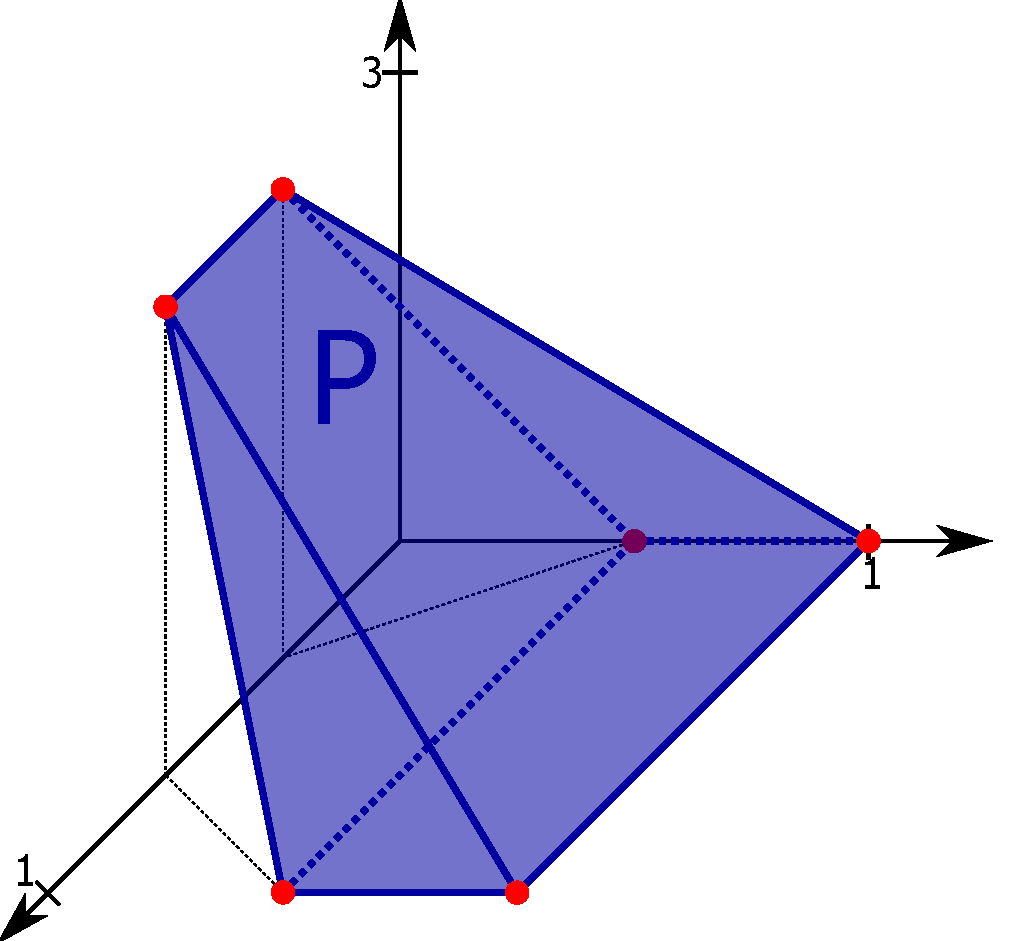
\includegraphics[width=\linewidth]{figs/3dpoly.pdf}
    \end{column}
    \end{columns}
\end{frame}

\begin{frame}
    \frametitle{Example}

    \small
    \begin{columns}
    \begin{column}{.3\textwidth}
    Let $P$
    \begin{align*}
        \left\{
        \begin{aligned}
        x_1 + 2x_2 &\leq 6 \\
        2x_1 + x_2 &\leq 6 \\
        x_1 &\geq 0 \\
        x_2 &\geq 0 
        \end{aligned}
        \right.
    \end{align*}
    be a polyhedron in $\R^2$.
    \begin{align*}
        \highlight[AlertOrange]{$\tilde A$} =
        \begin{bmatrix}
            1  & 2   \\
            2  & 1   \\
            -1 & 0   \\
            0  & -1
        \end{bmatrix},
        \highlight[UniBlue]{$\tilde b$} = 
        \begin{bmatrix}
            6 \\ 6 \\ 0 \\ 0    
        \end{bmatrix}
    \end{align*}
    \end{column}
    \begin{column}{.7\textwidth}
        \centering
    \begin{tikzpicture}[>=latex,scale=1.3]
        % draw grid
        \draw[gray,very thin] (-.9,-.9) grid (4.5,4.5);
        \node[circle,fill=UniBlue,inner sep=3pt, "{$(0,0)$}" below left] at (0,0) (O) {};
        \node[circle,fill=UniBlue,inner sep=3pt, "{$(3,0)$}" below] at (3,0) (A) {};
        \node[circle,fill=UniBlue,inner sep=3pt, "{$(2,2)$}" above right] at (2,2) (B) {};
        \node[circle,fill=UniBlue,inner sep=3pt, "{$(0,3)$}" above left] at (0,3) (C) {};
        \begin{scope}[on background layer]
            \draw[->,very thick] (-1, 0) -- (4.5,0) node[above] {$x_1$};
            \draw[->,very thick] (0 ,-1) -- (0,4.5) node[left ] {$x_2$};
            \draw[UniBlue, very thick, fill=UniBlue!10] (O.center) -- (A.center) -- (B.center) -- (C.center) -- cycle;
        \end{scope}
        \path (O) -- node[UniBlue,midway,below]{$x_2 \geq 0$} (A);
        \path (A) -- node[UniBlue,midway,above,sloped]{$2x_1 + x_2 \leq 6$} (B);
        \path (B) -- node[UniBlue,midway,above,sloped]{$x_1 + 2x_2 \leq 6$} (C);
        \path (O) -- node[UniBlue,midway,left]{$x_1 \geq 0$} (C);
        \node[UniBlue] at (1,1) {\large $P$};
    \end{tikzpicture}
    \end{column}
    \end{columns}
\end{frame}

%%%%%%%%%%%%%%%%%%%%%%%%%%%%%%%%%%%%%%%%%%%%%%%%%%
\section{Integral polyhedra and totally unimodular matrices}
\againframe<4|handout:0>{outline}
%%%%%%%%%%%%%%%%%%%%%%%%%%%%%%%%%%%%%%%%%%%%%%%%%%
\begin{frame}
    \frametitle{Solving combinatorial optimization with LP?}

    \begin{enumerate}
        \setlength{\itemsep}{1em}
        \item Formulate a combinatorial optimization problem as a \alert{0--1 integer program (IP)}.
        \item Solve the LP obtained by dropping the 0--1 constraints of the IP.
        \item If we got an $\{0,1\}$-LP solution, then it is also an optimum of the original IP, so the problem is solved (lucky!).
    \end{enumerate}

    \vfill
    A sufficient condition for this to work: \alert{total unimodularity}
\end{frame}

\begin{frame}<1-3>
    \frametitle{Example: Bipartite matching}

    \small
    \begin{columns}[T]
    \begin{column}{.6\textwidth}
        \begin{block}{Weighted bipartite matching problem}
            \structure{Input} $G=(V; E)$: a bipartite graph, \\ edge weights $w_e$ ($e \in E$) \\
            \structure{Output} A maximum-weight matching $M$ of $G$
        \end{block}


        \begin{block}<2->{\alt<2>{IP}{LP} formulation}
            \setlength{\abovedisplayskip}{0pt}
        \begin{alignat*}{2}
            \text{maximize} & \quad  \sum_{e \in E} w_e x_e \\
            \text{subject to} & \quad \sum_{e \in \delta(i)} x_e \leq 1 & \quad (i \in V) \\
            & \quad \alt<2>{x_e \in \{0,1\}}{} \only<3>{{\color{AlertOrange} x_e \geq 0}} & \quad (e \in E)
        \end{alignat*}
        \end{block}
        \only<2>{\footnotesize $\delta(i)$: the set of edges incident to vertex $i$}
    \end{column}
    \begin{column}{.4\textwidth}
        \centering
        \tikz{
            \graph[nodes={mynodes}, edges={myedges}, grow right=4em]{
            subgraph I_nm [V={1,2,3}, W={4,5}];
            1 -- {4,5};
            2 -- {4,5};
            3 -- {4};
            % matching
            {[edges={mypath}] {1,2} -- {4,5}; }
        };
        }
        \footnotesize
        \onslide<2->
        \begin{alignat*}{3}
            &\text{max}\quad  &&  w^\top x  \\
            &\text{s.t.}\quad  && x_{14} + x_{15}  &&\leq 1 \\
            & && x_{24} + x_{25}  &&\leq 1  \\
            & && x_{34}  &&\leq 1  \\
            & && x_{14} + x_{24} + x_{34} &&\leq 1  \\
            & && x_{15} + x_{25} &&\leq 1  \\
            & && 
            \only<3->{\color{AlertOrange}} x_{14}, x_{15}, x_{24}, x_{25}, x_{34} && \alt<2>{\in \{0, 1\} }{\color{AlertOrange}\geq 0}
        \end{alignat*}
    \end{column}
    \end{columns}
    \bigskip
    \onslide<3->{\structure{Goal:} Total unimodularity of the coefficient matrix ensures an LP optimal solution with \textbf{0--1} entries!}
\end{frame}


\begin{frame}
    \frametitle{Totally unimodular matrices}
    \begin{definition}[Totally unimodular matrix]
        A matrix $A$ is \alert{totally unimodular}
        $\defiff$ every subdeterminant of $A$ is either $0$ or $\pm 1$.
    \end{definition}

    \begin{example}
        \[
            \begin{bmatrix}
                1 & 0 \\
                0 & 1
            \end{bmatrix},
            \begin{bmatrix}
                -1 &  1 &  0 & 0  & -1 \\
                1  &  0 &  0 & -1 & 0  \\
                0  & -1 &  1 & 0  & 0  \\
                0  &  0 & -1 & 1  & 1  
            \end{bmatrix} 
        \]
    \end{example}
\end{frame}

\begin{frame}
    \frametitle{Example: Bipartite matching}
    
    \small
    \begin{columns}[T]
    \begin{column}{.67\textwidth}
    \begin{lemma}
    The coefficient matrix $A$ of the LP for bipartite matching is totally unimodular.
    \end{lemma}

    \begin{proof}<2->
    We prove by induction on $k$ that every $k \times k$ subdeterminant belongs to $\{0, \pm 1\}$.

    For $k=1$, this is trivial because every entry of $A$ is $0$ or $1$.

    Let $k>1$, and consider a $k \times k$ submatrix $A'$.
    \footnotesize
   \begin{itemize}
    \item<3-> If $A'$ has a zero column, then $\det A'=0$.
    \item<4-> If $A'$ has a column with single $1$, Laplace expansion gives $\det A'=\pm\det A''$ for a $(k-1)\times(k-1)$ submatrix $A''$. By the induction hypothesis, $\det A''\in\{0,\pm1\}$.
    \item<5-> Otherwise, every column has two $1$s. Let $v$ assign $+1$ to all left vertices and $-1$ to all right vertices. Then $vA'=0$, so $A'$ is singular and $\det A'=0$. \qed
   \end{itemize} 
    \end{proof}
    \end{column}
    \begin{column}{.3\textwidth}
        \centering
        \tikz{
            \graph[nodes={mynodes}, edges={myedges}, grow right=4em]{
            subgraph I_nm [V={1,2,3}, W={4,5}];
            1 -- {4,5};
            2 -- {4,5};
            3 -- {4};
        };
        }
        \footnotesize
    \[
        \begin{bNiceMatrix}[first-col=true, first-row=true]
            & x_{14} & x_{15} & x_{24} & x_{25} & x_{34} \\
          1 & 1 & 1 & 0 & 0 & 0 \\
          2 & 0 & 0 & 1 & 1 & 0 \\
          3 & 0 & 0 & 0 & 0 & 1 \\ \hline    
          4 & 1 & 0 & 1 & 0 & 1 \\     
          5 & 0 & 1 & 0 & 1 & 0    
        \end{bNiceMatrix}
    \]
    \end{column}
    \end{columns}

    

\end{frame}


\begin{frame}
    \frametitle{Integral polyhedra}

     \begin{definition}[Integral polyhedron]
         A polyhedron is \alert{integral} $\defiff$ Each extreme point is an integral vector.
    \end{definition}
    
    \small
    \begin{columns}[T]
    \begin{column}{.5\textwidth}
        \centering
    \begin{tikzpicture}[>=latex,scale=1.0]
        % draw grid
        \draw[gray,very thin] (-.9,-.9) grid (4.5,3.5);
        \node[circle,fill=UniBlue,inner sep=3pt] at (0,0) (O) {};
        \node[circle,fill=UniBlue,inner sep=3pt] at (3,0) (A) {};
        \node[circle,fill=UniBlue,inner sep=3pt] at (2,2) (B) {};
        \node[circle,fill=UniBlue,inner sep=3pt] at (0,3) (C) {};
        \begin{scope}[on background layer]
            \draw[->,very thick] (-1, 0) -- (4.5,0) node[above] {$x_1$};
            \draw[->,very thick] (0 ,-1) -- (0,3.5) node[left ] {$x_2$};
            \draw[UniBlue, very thick, fill=UniBlue!10] (O.center) -- (A.center) -- (B.center) -- (C.center) -- cycle;
        \end{scope}
    \end{tikzpicture}
    \\ Integral polyhedron
    \end{column}
    \begin{column}{.5\textwidth}
        \centering
    \begin{tikzpicture}[>=latex,scale=1.0]
        % draw grid
        \draw[gray,very thin] (-.9,-.9) grid (4.5,3.5);
        \node[circle,fill=UniBlue,inner sep=3pt] at (0,0) (O) {};
        \node[circle,fill=UniBlue,inner sep=3pt] at (3,0) (A) {};
        \node[circle,fill=AlertOrange,inner sep=3pt] at (2.5,2.5) (B) {};
        \node[circle,fill=UniBlue,inner sep=3pt] at (0,3) (C) {};
        \begin{scope}[on background layer]
            \draw[->,very thick] (-1, 0) -- (4.5,0) node[above] {$x_1$};
            \draw[->,very thick] (0 ,-1) -- (0,3.5) node[left ] {$x_2$};
            \draw[UniBlue, very thick, fill=UniBlue!10] (O.center) -- (A.center) -- (B.center) -- (C.center) -- cycle;
        \end{scope}
    \end{tikzpicture}
    \\ Non-integral polyhedron
    \end{column}
    \end{columns}
\end{frame}

\begin{frame}
    \frametitle{TU matrices and integral polyhedra}

    \small

    \begin{theorem}
        For a totally unimodular matrix $A$ and an integral vector $b$, the polyhedron
        $
        P = \{ x \in \R^n : Ax \leq b, \, x \geq 0 \} 
        $
    is integral.
    \end{theorem}
    
    \pause
    \begin{proof}
    Let $x$ be any extreme point of $P$. There are a nonsingular submatrix $A'$ and a subvector $b'$, obtained by selecting $n$ rows from $(\tilde A, \tilde b)$, such that $x = (A')^{-1}b'$.

    \pause
    \bigskip
    By Cramer's rule,
    \[
        (A')^{-1}_{ij} = \frac{\Delta_{j,i} A'}{\det A'} \in \{0,\pm 1\}
    \]
    {\footnotesize Here, $\Delta_{j,i} A'$ is the $(j,i)$-cofactor of $A'$.}

    \bigskip
    Since $b'$ is integral, $(A')^{-1}b'$ is also integral.
    \end{proof}
\end{frame}

\begin{frame}
    \frametitle{Total unimodularity and integrality of LP}
    
    \begin{columns}[T]
    \begin{column}{.75\textwidth}
    \begin{theorem}[]
        Let $A$ be a totally unimodular matrix and $b$ an integral vector.
        If (P) has an optimal solution, then it has an optimal solution that is an \textbf{integral vector}.
    \end{theorem}
    \end{column}
    \begin{column}{.2\textwidth}
        \footnotesize
    \begin{primal}
        \setlength{\abovedisplayskip}{0pt}
        \begin{alignat*}{2}
            \text{max} & \quad  c^\top x \\
            \text{s.t.} & \quad A x \leq b  \\
            & \quad x \geq 0 
        \end{alignat*}
    \end{primal}
    \end{column}
    \end{columns}

    \pause \vfill
    \begin{proof}
    By the preceding theorem, the feasible region $P$ of (P) is an integral polyhedron.
    Since (P) has an optimal solution, it has an optimal solution that is an extreme point of $P$.
    By the definition of an integral polyhedron, this solution is an integral vector.
    \end{proof}
\end{frame}

\end{document}